% Fixing: Too many math alphabets used in version normal.
\newcommand\hmmax{0}
\newcommand\bmmax{0}
\documentclass[12pt]{article}
\usepackage[left=1.0cm,top=1.5cm,right=1.0cm,bottom=1.5cm]{geometry}
\usepackage{parskip}
\usepackage{enumitem}
\usepackage[numbers]{natbib}
\usepackage{trimclip}
\makeatletter
\DeclareRobustCommand{\circbullet}{\mathbin{\vphantom{\circ}\text{\circbullet@}}}
\newcommand{\circbullet@}{%
  \check@mathfonts
  \m@th\ooalign{%
    \clipbox{0 0 0 {\dimexpr\height-\fontdimen22\textfont2}}{$\bullet$}\cr
    $\circ$\cr
  }%
}
\DeclareRobustCommand{\bulletcirc}{\mathbin{\text{\bulletcirc@}}}
\newcommand{\bulletcirc@}{%
  \check@mathfonts
  \m@th\ooalign{%
    \raisebox{\fontdimen22\textfont2}{\clipbox{0 {\fontdimen22\textfont2} 0 0}{$\bullet$}}\cr
    $\circ$\cr
  }%
}
\makeatother

% https://tex.stackexchange.com/questions/648845/sans-serif-uppercase-greek-no-longer-showing-in-acmart
\DeclareMathAlphabet{\mathsf}{OT1}{LibertinusSans-LF}{m}{n}
\SetMathAlphabet{\mathsf}{bold}{OT1}{LibertinusSans-LF}{bx}{n}
\DeclareMathAlphabet{\mathtt}{OT1}{lmtt}{m}{n}
\SetMathAlphabet{\mathtt}{bold}{OT1}{lmtt}{bx}{n}


\usetikzlibrary{calc,decorations.pathmorphing,shapes,positioning}
\newcounter{sarrow}
\newcommand\xrsquigarrow[1]{%
\stepcounter{sarrow}%
\mathrel{\begin{tikzpicture}[baseline= {( $ (current bounding box.south) + (0,-0.5ex) $ )}]
\node[inner sep=.5ex] (\thesarrow) {$\scriptstyle #1$};
\path[draw,<-,decorate,
  decoration={zigzag,amplitude=0.7pt,segment length=1.2mm,pre=lineto,pre length=4pt}]
    (\thesarrow.south east) -- (\thesarrow.south west);
\end{tikzpicture}}%
}
\makeatletter
\newcommand{\xRightarrow}[2][]{\ext@arrow 0359\Rightarrowfill@{#1}{#2}}
\makeatother

\newcommand{\thmref}[1]{\cref{#1}~(\nameref{#1})}
\newcommand{\Thmref}[1]{\Cref{#1}~(\nameref{#1})}

%%%%
% TODO macros
\newcommand{\MK}[1]{\todo[color=orange!30]{TODO: #1}}
\newcommand{\MKin}[1]{\todo[color=orange!30,inline]{TODO: #1}}
\newcommand{\MP}[1]{\todo[color=blue!30]{TODO: #1}}
\newcommand{\MPin}[1]{\todo[color=blue!30,inline]{TODO: #1}}
\newcommand{\hltt}[1]{\begin{center}\fbox{\color{green}\large{#1}}\end{center}}

% Approx
\newcommand{\pages}[1]{}%\xspace\todo{\textbf{($\sim$#1 pages)}\xspace}}

%%%%
% Colors
\newcommand{\neutcol}[0]{black}
\newcommand{\stlccol}[0]{RoyalBlue}
\newcommand{\irccol}[0]{Apricot}
\newcommand{\ulccol}[0]{RedOrange}
\newcommand{\objcol}[0]{Emerald} %CarnationPink}
\newcommand{\commoncol}[0]{black}

\newcommand{\col}[2]{\ensuremath{{\color{#1}{#2}}}}

\newcommand{\com}[1]{\ensuremath\mathit{\col{\neutcol}{#1}}}
\newcommand{\src}[1]{\ensuremath\mathsf{\col{\stlccol}{#1}}}
\newcommand{\irl}[1]{\ensuremath\mathit{\col{\irccol}{#1}}}
\newcommand{\trg}[1]{\ensuremath\mathbf{\col{\ulccol}{#1}}}
\newcommand{\obj}[1]{\ensuremath\mathtt{\col{\objcol}{#1}}}

%%%%
% Text Decorations
\newcommand\BrText[2]{%
  \par\smallskip
   \noindent\makebox[\textwidth][r]{$\text{\scriptsize #1}\left\{
    \begin{minipage}{\textwidth}
    #2
    \end{minipage}
  \right.\nulldelimiterspace=0pt$}\par\smallskip
}
\newcommand{\mi}[1]{\ensuremath{\mathit{#1}}}
\newcommand{\mr}[1]{\ensuremath{\mathrm{#1}}}
\newcommand{\mt}[1]{\ensuremath{\texttt{#1}}}
\newcommand{\mtt}[1]{\ensuremath{\mathtt{#1}}}
\newcommand{\mf}[1]{\ensuremath{\mathbf{#1}}}
\newcommand{\mk}[1]{\ensuremath{\mathfrak{#1}}}
\newcommand{\mc}[1]{\ensuremath{\mathcal{#1}}}
\newcommand{\ms}[1]{\ensuremath{\mathsf{#1}}}
\newcommand{\mb}[1]{\ensuremath{\mathbb{#1}}}
\newcommand{\msc}[1]{\ensuremath{\mathscr{#1}}}

\newcommand{\bul}[1]{{\setulcolor{RoyalBlue}\ul{#1}}}
\newcommand{\rul}[1]{{\setulcolor{RedOrange}\ul{#1}}}
\newcommand{\iul}[1]{{\setulcolor{Apricot}\ul{#1}}}
\newcommand{\oul}[1]{{\setulcolor{Emerald}\ul{#1}}}
\newcommand{\pul}[1]{{\setulcolor{CarnationPink}\ul{#1}}}

\newcommand{\lock}{\ensuremath\text{\scriptsize\faIcon{lock}}}
\newcommand{\unlock}{\ensuremath\text{\scriptsize\faIcon{lock-open}}}

\newcommand{\tup}[2]{\ensuremath (#1 %
  \readlist\myterms{#2}%
  \foreachitem\x\in\myterms{;\x}%
  )%
}

\newcommand{\isdef}[0]{\ensuremath{\mathrel{\overset{\makebox[0pt]{\mbox{\normalfont\tiny\sffamily def}}}{=}}}}

%%%%
% List of contributions
\newcounter{contrib}
\newcommand{\contribnum}[0]{\stepcounter{contrib}{\arabic{contrib}}.~}
\newcommand{\contribution}[1]{\smallskip\noindent\textbf{{#1.}\xspace}}

%%%%
% A symbol for Coq-verified theorems.
\newcommand{\BareCoqSymbol}{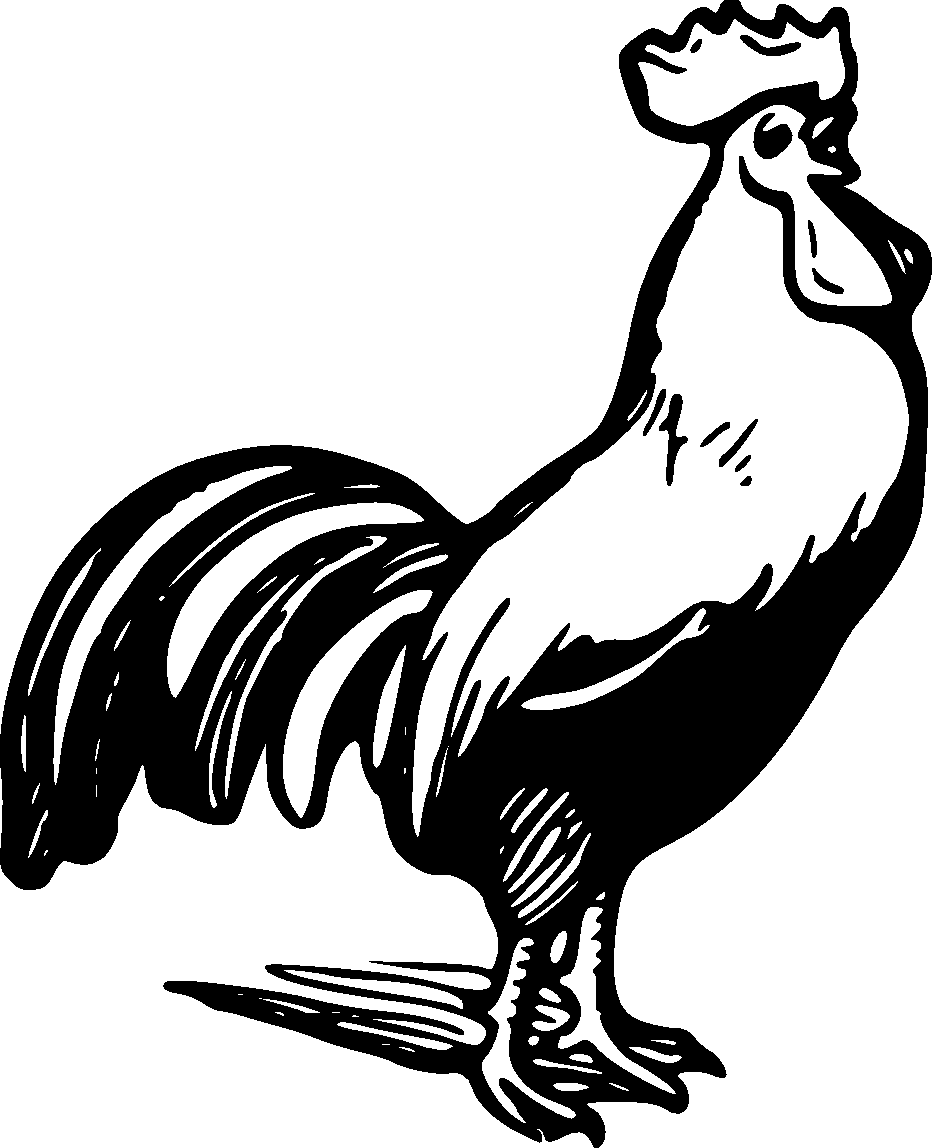
\includegraphics[height=0.9em]{coq.pdf}}
\newcommand{\CoqSymbol}{\raisebox{-.2ex}{\BareCoqSymbol\,}}
\newcommand{\Coqed}{\hfill\CoqSymbol}

\newcommand{\BareInvCoqSymbol}{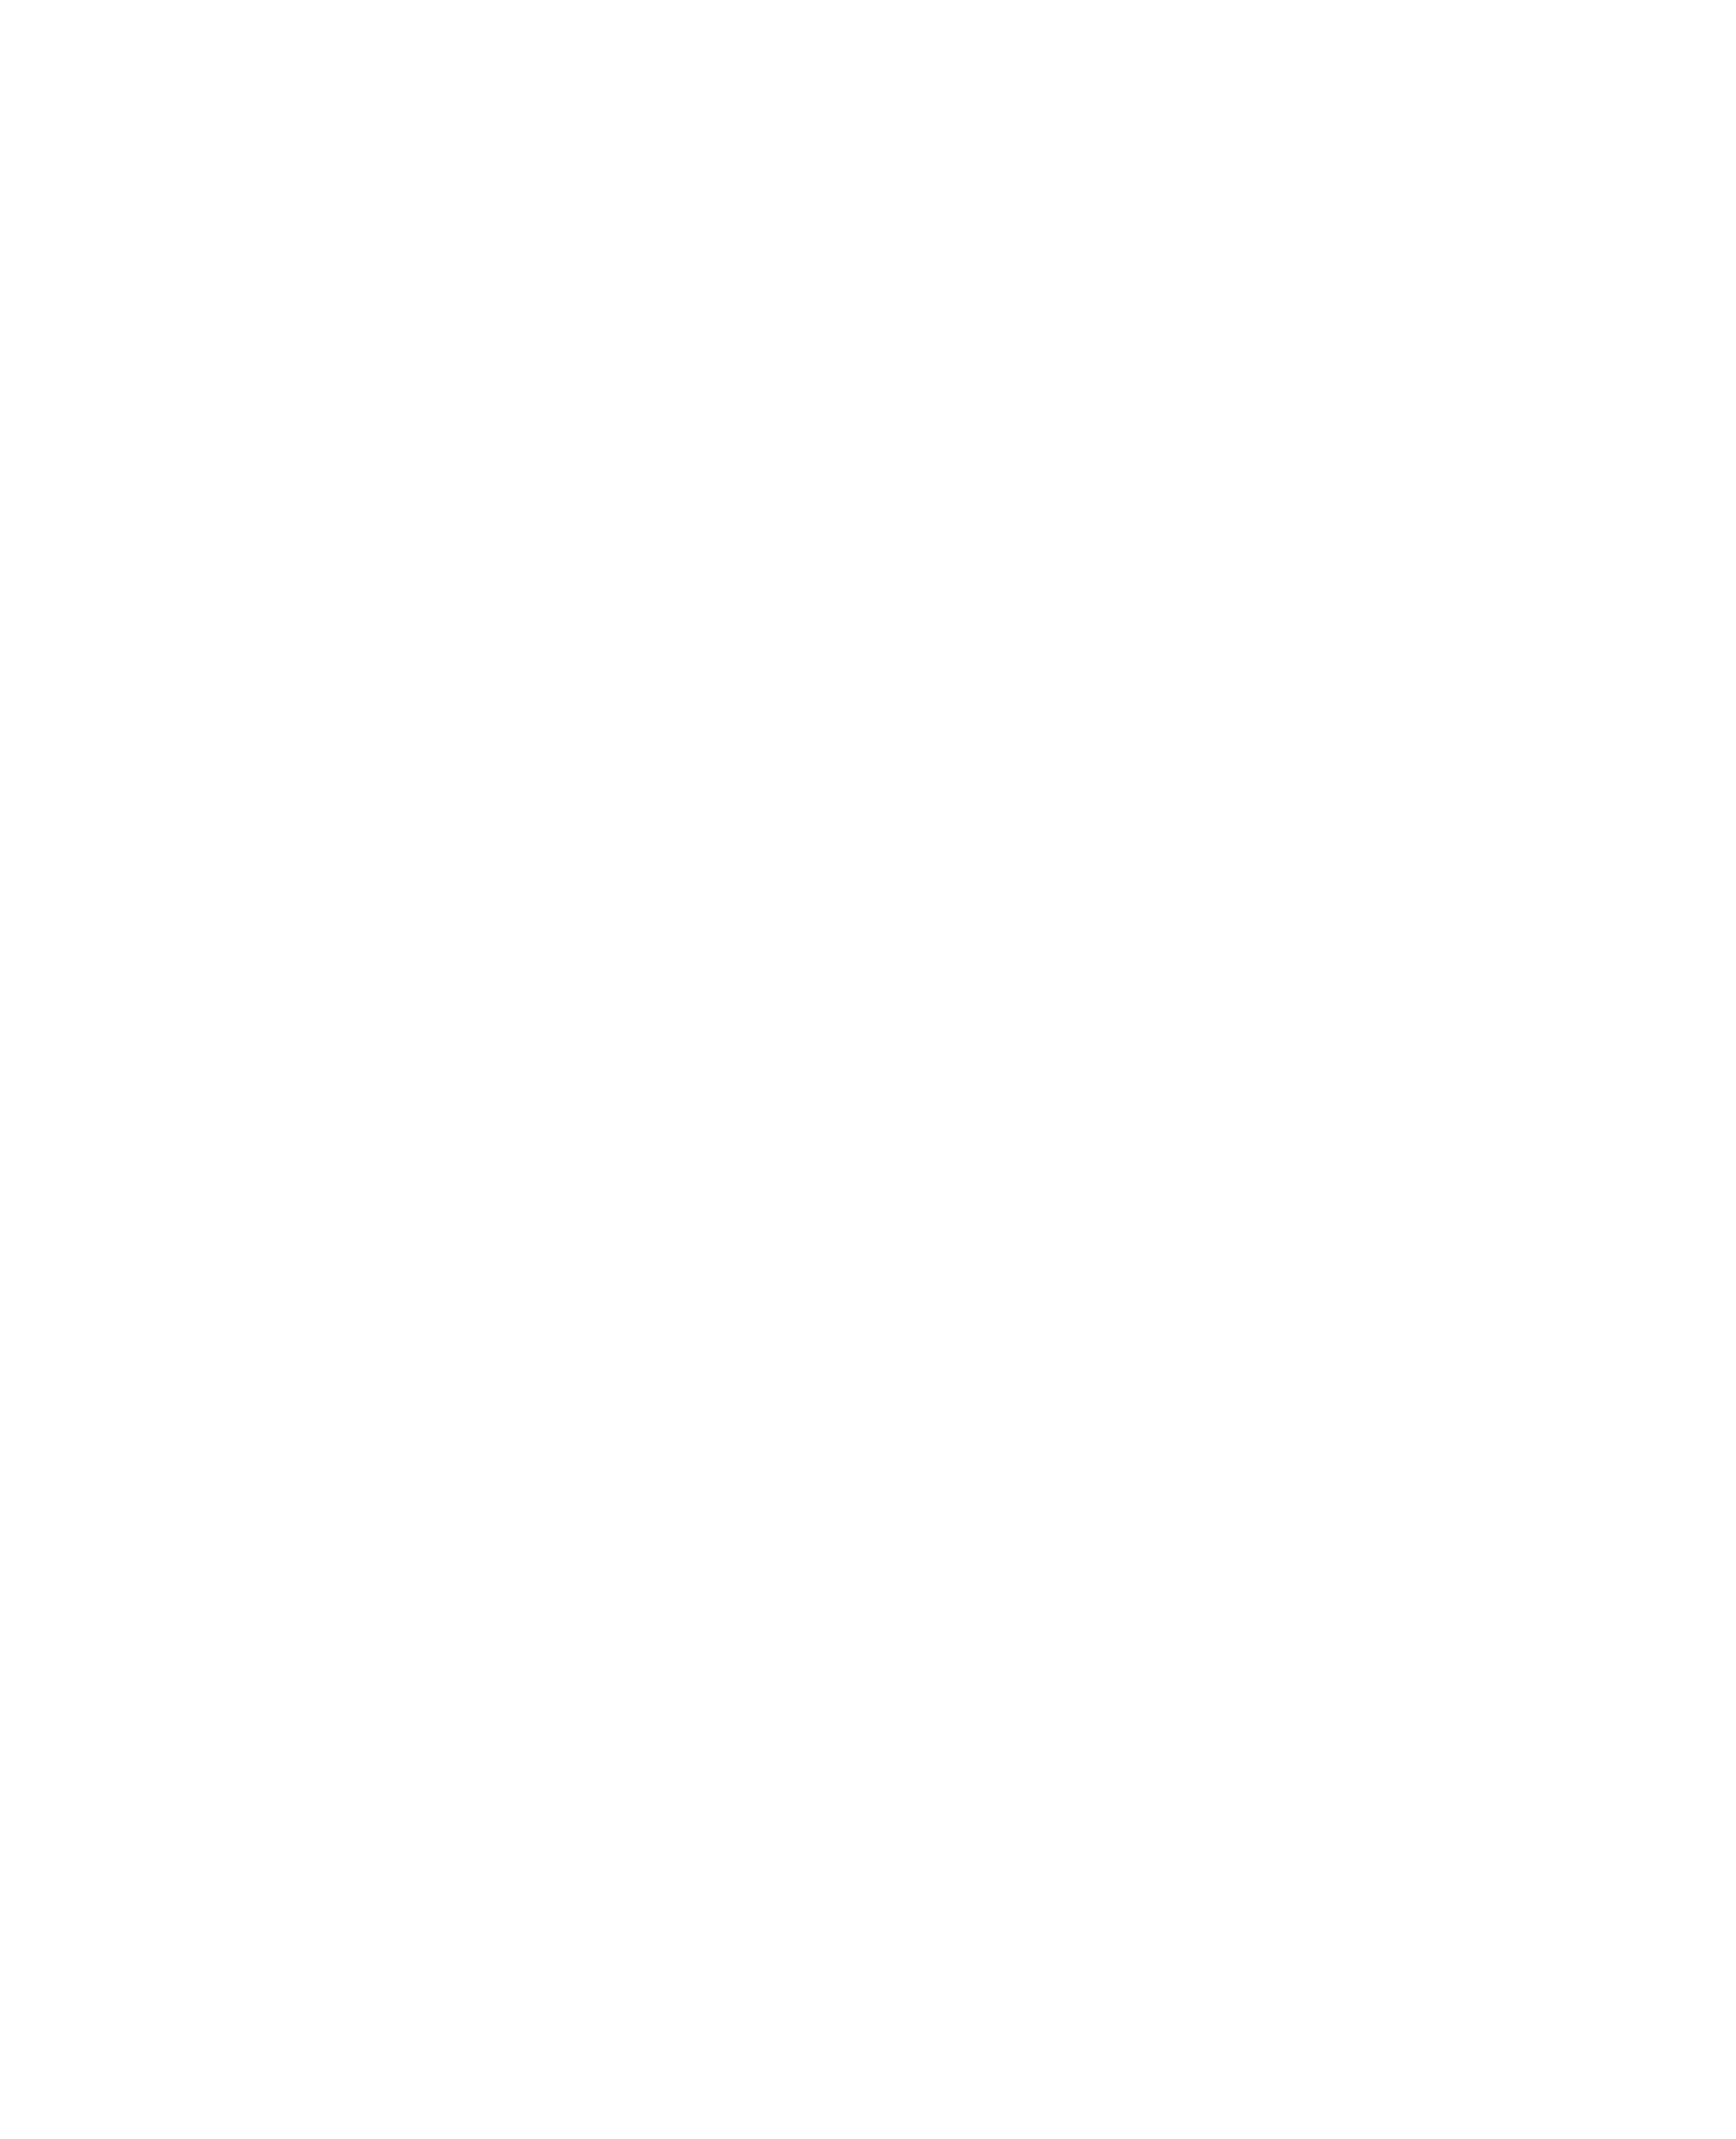
\includegraphics[height=0.9em]{inv_coq.png}}
\newcommand{\InvCoqSymbol}{\raisebox{-.2ex}{\BareInvCoqSymbol\,}}

%%%%
% Typerules
\newcommand{\textgraybox}[1]{\boxed{#1}}
\newdimen\zzfontsz
\newcommand{\fontsz}[2]{\zzfontsz=#1%
{\fontsize{\zzfontsz}{1.2\zzfontsz}\selectfont{#2}}}
\newcommand{\mathsz}[2]{\text{\fontsz{#1}{$#2$}}}
\newcommand{\instsymColon}{%
     \raisebox{-0.09ex}{\text{\normalfont{:}}}}
\newcommand{\judgboxfontsize}[1]{%
        \mathsz{11pt}{#1}%
}
\newcommand{\judgbox}[2]{%
      {\raggedright \textgraybox{\ensuremath{\judgboxfontsize{#1}}}\!%
        \fontsz{9pt}{\begin{tabular}[c]{l} #2 \end{tabular}} %
}}
\newcounter{typerule}
\crefname{typerule}{rule}{rules}

\newcommand{\typeruleInt}[5]{%
	\def\thetyperule{#1}%
	\refstepcounter{typerule}%
	\label{tr:#4}%
	%
  \ensuremath{\begin{array}{c}#5 \inference{#2}{#3}\end{array}}
}
\newcommand{\typerule}[4]{%
  \typeruleInt{#1}{#2}{#3}{#4}{\textsf{\scriptsize ({#1})} \\      }
}
\newcommand{\typerulenolabel}[3]{%
	\def\thetyperule{#1}%
	\refstepcounter{typerule}%
  \ensuremath{\begin{array}{c} \inference{#2}{#3}\end{array}}
}
\newcommand{\typerulederiv}[3]{%
  \ensuremath{\begin{array}{c} \inference{#2}{#3} #1\end{array}}
}

%%%%
% Language-specific definitions
% names of properties
\newcommand{\tmssafe}{\ensuremath\operatorname{tms}}
\newcommand{\smssafe}{\ensuremath\operatorname{sms}}
\newcommand{\mssafe}{\ensuremath\operatorname{ms}}
\newcommand{\scctsafe}{\ensuremath\operatorname{scct}}
\newcommand{\msscctsafe}{\ensuremath\operatorname{msscct}}

% Languages
\newcommand{\Ltms}{\ensuremath\src{L_{\tmssafe}}}
\newcommand{\Ltrg}{\ensuremath\trg{L}}
\newcommand{\Lms}{\ensuremath\irl{L_{\mssafe}}}
\newcommand{\Lscct}{\ensuremath\obj{L_{\scctsafe}}}

% Traces
\newcommand{\event}[1][]{a#1}
\newcommand{\absevent}[1][]{\ensuremath\bm{\event[#1]}}
\newcommand{\emptyevent}{\ensuremath\varepsilon}
\newcommand{\trace}[1][]{\ensuremath\overline{a#1}}
\newcommand{\class}[1][]{\ensuremath\mb{C}}
\newcommand{\lift}[1]{\ensuremath\lfloor\xspace{#1}\xspace\rfloor}
\newcommand{\hole}[1]{\ensuremath{\left[#1\right]}}
\newcommand{\ev}[1]{\text{#1}}
\newcommand{\absev}[1]{\ensuremath\bm{#1}}
\newcommand{\abstrace}[1][]{\ensuremath\bm{\trace[]}#1}
\newcommand{\absterm}{\ensuremath\lightning{\kern-5.5pt}\lightning}

% Trace Relations
\newcommand{\traceagree}[4][^*]{\ensuremath{#3}\cong_{#2}#1{#4}}
\newcommand{\tmstraceagree}[3][^*]{\traceagree[#1]{\tmssafe}{#2}{#3}}
\newcommand{\smstraceagree}[3][^*]{\traceagree[#1]{\smssafe}{#2}{#3}}
\newcommand{\mstraceagree}[3][^*]{\traceagree[#1]{\mssafe}{#2}{#3}}
\newcommand{\sccttraceagree}[3][^*]{\traceagree[#1]{\scctsafe}{#2}{#3}}

% Monitors
\newcommand{\monitor}[1][]{\ensuremath T#1}
\newcommand{\tmsmonitor}[1][]{\monitor[_{TMS}{#1}]}
\newcommand{\smsmonitor}[1][]{\monitor[_{SMS}{#1}]}
\newcommand{\scctmonitor}[1][]{\monitor[_{sCCT}{#1}]}
\newcommand{\msmonitor}[1][]{\monitor[_{MS}{#1}]}
\newcommand{\monitorcheck}[4][{\kern-3.5pt}^*]{%
  \vdash\xspace{#2}\xspace \xrsquigarrow{#4}{#1}\xspace{#3}\xspace%
}
\newcommand{\monsafe}[2]{\ensuremath\vdash_{mon}{#1}:{#2}}

\newcommand{\abssecuritytag}[1][]{\ensuremath\bm{\sigma}#1}

\newcommand{\montmssafe}[1]{\monsafe{#1}{\tmssafe}}
\newcommand{\monsmssafe}[1]{\monsafe{#1}{\smssafe}}
\newcommand{\monmssafe}[1]{\monsafe{#1}{\mssafe}}
\newcommand{\monscctsafe}[1]{\monsafe{#1}{\scctsafe}}
\newcommand{\monmsscctsafe}[1]{\monsafe{#1}{\msscctsafe}}

% Languages
\newcommand{\LTMS}{\src{L_{TMS}}}
\newcommand{\LT}{\trg{L}}
\newcommand{\LMS}{\irl{L_{MS}}}
\newcommand{\LCCT}{\obj{L_{sCCT}}}

\newcommand{\bnfdef}{\ensuremath{\mathrel{::=}}}

% Substitution
\newcommand{\subst}[2]{\ensuremath \hole{#1\text{ for }#2}}
\newcommand{\substvar}[1][]{\ensuremath \gamma#1}
\newcommand{\substlist}[1][]{\ensuremath \overline{\gamma#1}}

\newcommand{\partialeval}[2]{\ensuremath \operatorname{\mathtt{mix}}(#1, #2)}

% Predefined Sets
\newcommand{\nat}{\ensuremath\mb{N}}

% Types
\newcommand{\natt}{\ensuremath\mb{N}_t\xspace}
\newcommand{\ptrqual}[1][]{\ensuremath\xspace q#1\xspace}
\newcommand{\fullq}{1\xspace}
\newcommand{\halfq}{\sfrac{1}{2}\xspace}
\newcommand{\ptrn}[1][\ptrqual]{\ensuremath\xspace ref_{#1}\ \natt\xspace}
\newcommand{\wptr}{\ensuremath\ptrn[\halfq]\xspace}
\newcommand{\ptr}{\ensuremath\ptrn[\fullq]\xspace}
\newcommand{\type}[1][]{\ensuremath\tau#1\xspace}
\newcommand{\typenv}[1][]{\ensuremath\Gamma#1\xspace}

% Terms
\newcommand{\wrapkeyword}[2][]{\ensuremath{#1{#2}}}
\newcommand{\expr}[1][]{e#1\xspace}
\newcommand{\ectx}[1][]{K#1\xspace}
\newcommand{\finalexpr}[1][]{f#1\xspace}
\newcommand{\valueexpr}[1][]{v#1\xspace}
\newcommand{\lbinop}[3][]{\ensuremath {#2}{#1{\oplus}}{#3}\xspace}
\newcommand{\lget}[3][]{\ensuremath #2{#1{[}}{#3}{#1{]}}\xspace}
\newcommand{\lset}[4][]{\ensuremath #2{#1{[}}{#3}{#1{]\leftarrow}}#4\xspace}
\newcommand{\lnew}[3][]{\ensuremath \wrapkeyword[#1]{new}\ #2\ {#1{[}}#3{#1{]}}\xspace}
\newcommand{\llet}[4][]{\ensuremath \wrapkeyword[#1]{let}\ #2 {#1{=}} #3\ \wrapkeyword[#1]{in}\ #4\xspace}
\newcommand{\ldelete}[2][]{\ensuremath \wrapkeyword[#1]{delete}\ #2\xspace}
\newcommand{\lreturn}[2][]{\ensuremath \wrapkeyword[#1]{return}\ #2\xspace}
\newcommand{\lcall}[3][]{\ensuremath \wrapkeyword[#1]{call}\ #2\ #3\xspace}
\newcommand{\lifz}[4][]{\ensuremath \wrapkeyword[#1]{ifz}\ #2\ \wrapkeyword[#1]{then}\ #3\ \wrapkeyword[#1]{else}\ #4\xspace}
\newcommand{\labort}[1][]{\ensuremath \wrapkeyword[#1]{abort()}\xspace}
\newcommand{\lispoisoned}[2][]{\ensuremath #2\ \wrapkeyword[#1]{is\ }{#1{\poisoned}}\xspace}
\newcommand{\lpair}[3][]{\ensuremath {#1{\langle}} #2 {#1{;}} #3 {#1{\rangle}} \xspace}
\newcommand{\lproja}[2][]{\ensuremath {#2}{#1{.0}} \xspace}
\newcommand{\lprojb}[2][]{\ensuremath {#2}{#1{.1}} \xspace}
\newcommand{\lhast}[3][]{\ensuremath {#2}\ \wrapkeyword[#1]{has}\ #3 \xspace}
\newcommand{\lwrdoit}[2][]{\ensuremath \wrapkeyword[#1]{wrdoit}\ #2\xspace}
\newcommand{\lrddoit}[3][]{\ensuremath \wrapkeyword[#1]{rddoit}\ #2\ \wrapkeyword[#1]{in}\ #3\xspace}
\newcommand{\function}[1][]{F#1\xspace}
\newcommand{\lfunction}[4][]{\ensuremath\wrapkeyword[#1]{fn}\ {#2}\ {#3}\ {#1{:=}}\ #4\xspace}
\newcommand{\prog}[3][]{\ensuremath\wrapkeyword[#1]{\langle}\ #2; #3\wrapkeyword[#1]{\rangle}\xspace}

% Compiler
\newcommand{\rtp}[2]{\ensuremath\vdash{#1}:{#2}}
\newcommand{\ccbase}[1][]{\ensuremath\gamma{#1}}
\newcommand{\cc}[3][]{\ensuremath{\ccbase[#1]}^{#2}_{#3}\xspace}
\newcommand{\cca}{\ensuremath\cc{\Ltms}{\Ltrg}}
\newcommand{\ccb}{\ensuremath\cc{\Ltrg}{\Lms}}
\newcommand{\ccdce}{\ensuremath\cc[_{\gls{dce}}]{\Lms}{\Lms}}
\newcommand{\cccf}{\ensuremath\cc[_{\gls{cf}}]{\Lms}{\Lms}}
\newcommand{\ccscct}{\ensuremath\cc{\Lms}{\Lscct}}
\newcommand{\ccmsscct}{\ensuremath\cc{\Ltms}{\Lscct}}

% Backtranslation
\newcommand{\backbase}[1][]{\ensuremath\wp#1}
\newcommand{\backt}[3][]{\ensuremath{}^{#2}_{#3}\backbase[#1]}

% Satisfaction
\newcommand{\contextvar}[1][]{C#1}
\newcommand{\progvar}[1][]{p#1}
\newcommand{\wholeprogvar}[1][]{w#1}
\renewcommand{\class}[1][]{\mathbb{C}#1}
\newcommand{\link}[2]{\ensuremath\operatorname{link}\left({#1};{#2}\right)}
\newcommand{\behav}[1]{\ensuremath\operatorname{behav}\left({#1}\right)}
\newcommand{\sat}[2]{\ensuremath\vdash{#1}:{#2}}
\newcommand{\rsat}[2]{\ensuremath\vdash_R{#1}:{#2}}

% State
\newcommand{\securitytag}[1][]{\ensuremath\sigma#1}
\newcommand{\sandboxtag}[1][]{t#1}
\newcommand{\ctx}{\text{ctx}}
\newcommand{\comp}{\text{comp}}
\newcommand{\loc}[1][]{\ensuremath l#1}
\newcommand{\poison}{\ensuremath\rho}
\newcommand{\poisoned}{\ensuremath\text{\Biohazard}}
\newcommand{\poisonless}{\ensuremath\square}
\newcommand{\store}[1][]{\ensuremath\Delta#1}
\newcommand{\storeel}[5]{\ensuremath #1\mapsto\tup{#2}{#3,#4,#5}}
\newcommand{\comm}[1][]{\ensuremath c#1}
\newcommand{\ctxtocomp}{\ensuremath\xspace ? \xspace}
\newcommand{\comptoctx}{\ensuremath\xspace ! \xspace}
\newcommand{\nocomm}{\ensuremath\xspace \varnothing \xspace}
\newcommand{\heap}[1][]{\ensuremath H#1}
\newcommand{\ectxstack}[1][]{\ensuremath\overline{\ectx#1}}
\newcommand{\library}[1][]{\ensuremath\Xi#1}
\newcommand{\commlib}[1][]{\ensuremath\xi#1}
\newcommand{\cfstate}[1][]{\ensuremath\Psi#1}
\newcommand{\memstate}[1][]{\ensuremath\Phi#1}
\newcommand{\statevar}[1][]{\ensuremath\Omega#1}
\newcommand{\rtt}[2]{\ensuremath #1 \triangleright #2}
\newcommand{\growh}[2]{\ensuremath #1 \ll #2}
\newcommand{\seth}[3]{\ensuremath #1(#2 \mapsto #3)}

% Various Judgements
\newcommand{\fresh}[2]{\ensuremath{#1}\vdash{#2}\xspace\operatorname{fresh}\xspace}
\newcommand{\tcheck}[3]{\ensuremath{#1}\vdash{#2}:{#3}\xspace}
\newcommand{\notowned}[1]{\ensuremath\vdash{#1}\xspace\operatorname{not-owned}\xspace}
\newcommand{\typenvsplit}[2]{\ensuremath {#1}\odot{#2}\xspace}
\newcommand{\hastype}[2]{\ensuremath{#1}:{#2}\xspace}
\newcommand{\inttype}[1]{\ensuremath\vdash{#1}\operatorname{int-\type}\xspace}

\newcommand{\thelocmap}{\ensuremath\delta\xspace}
\newcommand{\locmapsto}[2]{\ensuremath\thelocmap({#1})={#2}\xspace}

% Filters
\newcommand{\filter}[4][]{\ensuremath \operatorname{Proj}^{#1}_{#2}\left({#3}, {#4}\right)\xspace}
\newcommand{\msfilterLtms}[2][{\thelocmap}]{\ensuremath\filter[{\Ltms}]{}{#1}{#2}}
\newcommand{\msfilterLms}[2][{\thelocmap}]{\ensuremath\filter[{\Lms}]{}{#1}{#2}}
\newcommand{\msfilterL}[2][{\thelocmap}]{\ensuremath\filter[{\Ltrg}]{}{#1}{#2}}
\newcommand{\scctfilterLms}[2][{\thelocmap}]{\ensuremath\filter[{\Lms}]{}{#1}{#2}}
\newcommand{\scctfilterLscct}[2][{\thelocmap}]{\ensuremath\filter[{\Lscct}]{}{#1}{#2}}

% Steps
\newcommand{\isval}[1]{\ensuremath\vdash{#1}\xspace\operatorname{is-val}\xspace}
\newcommand{\runtimetermvar}[1][]{r#1}
\newcommand{\stepto}[4][{\kern-4.5pt}^*]{\ensuremath{#2}\xrightarrow{#4}{}\xspace{#1}\xspace{#3}\xspace}
\newcommand{\stepton}[4][n]{\ensuremath{#2}\xrightarrow{#4}{}{\kern-3.5pt}^{#1}\xspace{#3}\xspace}

\newcommand{\pstepto}[3]{\ensuremath{#1}\xrightarrow{#3}_p{}\xspace{#2}\xspace}
\newcommand{\estepto}[4][{\kern-4.5pt}^*]{\ensuremath{#2}\xrightarrow{#4}#1_{\operatorname{ectx}}\xspace{#3}\xspace}
\newcommand{\estepton}[4][n]{\ensuremath{#2}\xrightarrow{#4}_{\operatorname{ectx}}{}{\kern-14.5pt}^{#1\ \ \ \;}\xspace{#3}\xspace}
\newcommand{\progstepto}[3]{\ensuremath{#1}\xRightarrow{#3}{#2}}


\newcommand{\ccseqct}{\ensuremath\llbracket\cdot\rrbracket^{\text{seq}}_{\text{ct}}}
\newcommand{\ccseqmem}{\ensuremath\llbracket\cdot\rrbracket^{\text{seq}}_{\text{mem}}}
\newcommand{\ccspecmem}{\ensuremath\llbracket\cdot\rrbracket^{\text{spec}}_{\text{mem}}}
\newcommand{\ccspecct}{\ensuremath\llbracket\cdot\rrbracket^{\text{spec}}_{\text{ct}}}
\newcommand{\ccspecpathct}{\ensuremath\llbracket\cdot\rrbracket^{\text{spec}}_{\text{ct}}}
\newcommand{\ccseqarch}{\ensuremath\llbracket\cdot\rrbracket^{\text{seq}}_{\text{arch}}}
\newcommand{\ccspecarch}{\ensuremath\llbracket\cdot\rrbracket^{\text{spec}}_{\text{arch}}}
\newcommand{\ccseqspecctpc}{\ensuremath\llbracket\cdot\rrbracket^{\text{seq-spec}}_{\text{ct-pc}}}
\newcommand{\ccbot}{\ensuremath\llbracket\cdot\rrbracket_\top}

\newcommand{\partialsec}{\ensuremath\circbullet}
\newcommand{\fullsec}{\ensuremath\bullet}

\newcommand{\proven}{\ensuremath\checkmark}
\newcommand{\partiallyproven}{\ensuremath(\checkmark)}
\newcommand{\informal}{\ensuremath\times}

\newcommand{\specpht}{\ensuremath\text{PHT}}
\newcommand{\specssb}{\ensuremath\text{SSB}} %is this relevant?
\newcommand{\specrsb}{\ensuremath\text{RSB}}
\newcommand{\specbtb}{\ensuremath\text{BTB}}
\newcommand{\specstl}{\ensuremath\text{STL}}
\newcommand{\specpsf}{\ensuremath\text{PSF}}

\loadglsentries{acronyms}
\makeglossaries

\begin{document}

\begin{center}
  \begin{tabular}{|c|c|c|c|c|c|c|}
    \hline
    Ref. &
    Cont. &
    Variants &
    Mitigations &
    Proof &
    Security &
    Platform
    \\\hline
    %
    \cite{vassena2021blade} &
    \acrshort{ccspecct} &
    $\specpht,\specrsb$ &
    \acrshort{fi}, \acrshort{slh} &
    $\partiallyproven$ &
    $\fullsec$ &
    \acrshort{s}
    \\
    %
    \cite{elatali2024cmr} &
    \acrshort{ccspecct} &
    $\specpht,\specrsb$ &
    \acrshort{cmr} &
    $\informal$ &
    $\partialsec$ &
    \acrshort{hs}
    \\
    %
    \cite{yu2019stt} &
    \acrshort{ccspecarch} &
    $\specpht$ &
    \acrshort{dtt} &
    $\partiallyproven$ &
    $\partialsec$ &
    \acrshort{h}
    \\
    %
    \cite{lfence} &
    ? &
    $\specpht$ &
    \acrshort{fi} &
    $\informal$ &
    $\fullsec$ &
    \acrshort{s}
    \\
    %
    \cite{lfence} &
    ? &
    $\specssb$ &
    \acrshort{msr} &
    $\informal$ &
    $\fullsec$ &
    \acrshort{s}/\acrshort{h}
    \\
    %
    \cite{mosier2023serberus} &
    \acrshort{ccspecct} &
    $\specpht$, $\specbtb$, $\specrsb$, $\specstl$, $\specpsf$ &
    \acrshort{fi},\acrshort{iso},\acrshort{rz} &
    $\partiallyproven$ &
    $\fullsec$ &
    \acrshort{s}
    \\
    %
    \cite{narayan2021swivel} &
    \acrshort{ccspecmem} &
    $\specpht$, $\specbtb$, $\specrsb$, $\specstl$, $\specpsf$ &
    \acrshort{iso},\acrshort{sm},\acrshort{ri} &
    $\informal$ &
    $\fullsec$ &
    \acrshort{s}/\acrshort{h}
    \\
    %
    \cite{barber2019specshield} &
    \acrshort{ccspecmem} &
    $\specpht$, $\specbtb$, $\specssb$, $\specstl$ &
    - &
    $\informal$ &
    $\partialsec$ &
    \acrshort{hs}
    \\
    %
    \cite{weisse2019nda} &
    ? &
    $\specpht$, $\specbtb$, $\specrsb$, $\specssb$, $\specstl$ &
    - &
    $\informal$ &
    $\fullsec$ &
    \acrshort{hs}
    \\
    %
    \cite{schwarz2019context} &
    ? &
    $\specpht$, $\specbtb$, $\specrsb$, $\specssb$, $\specstl$ &
    \acrshort{ntmmap} &
    $\informal$ &
    $\fullsec$ &
    \acrshort{s}/\acrshort{h}
    \\
    %
    \cite{khasawneh2018safespec} &
    \acrshort{ccspecct} &
    $\specpht$, $\specbtb$ &
    \acrshort{sm} &
    $\informal$ &
    $\fullsec$ &
    \acrshort{h}
    \\
    %
    % authors claim compositionality with fencing and sandboxing
    % however, it's not robust: they assume all code to follow a certain scheme
    \cite{shen2019venkman} &
    \acrshort{ccspecct} &
    $\specbtb$, $\specrsb$ &
    \acrshort{fi},\acrshort{iso} &
    $\informal$ &
    $\fullsec$ &
    \acrshort{s}
    \\
    %
    % claim it combines well with safespec and invisspec (both are hardware)
    \cite{koruyeh2019speccfi} &
    \acrshort{ccspecct} &
    $\specbtb$, $\specrsb$ &
    \acrshort{cfi} &
    $\informal$ &
    $\fullsec$ &
    \acrshort{s}/\acrshort{h}
    \\
    %
    \cite{yan2018invisispec} &
    \acrshort{ccspecct} &
    $\specpht$, $\specbtb$, $\specrsb$, $\specssb$, $\specstl$  &
    \acrshort{iso} &
    $\informal$ &
    $\fullsec$ &
    \acrshort{h}
    \\
    %
    \cite{eleksenko2018bypass} &
    ? &
    $\specpht$ &
    \acrshort{add} &
    $\informal$ &
    ? &
    \acrshort{s}
    \\
    %
    \cite{slh} &
    ? &
    $\specpht$ &
    \acrshort{slh} &
    $\informal$ &
    $\partialsec$ & % may leak data accessed non-speculativey
                    % misses variable time instructions
    \acrshort{s}
    \\
    %
    \cite{patrignani2021exorcising} &
    \acrshort{ccspecct} &
    $\specpht$ &
    \acrshort{sslh} &
    $\proven$ &
    $\partialsec$ & % misses variable time instructions
    \acrshort{s}
    \\
    %
    \cite{zhang2023uslh} &
    \acrshort{ccspecct} &
    $\specpht$ &
    \acrshort{uslh} &
    $\proven$ &
    $\fullsec$ &
    \acrshort{s}
    \\
    %
    \cite{taram2019csf} &
    \acrshort{ccspecct} &
    $\specpht$, $\specrsb$, $\specbtb$ &
    \acrshort{fi} &
    $\informal$ &
    $\fullsec$ &
    \acrshort{h}
    \\
    %
    \hline
  \end{tabular}
\end{center}

\footnotetext{
The above table uses execution modes \gls{seq}, \gls{seq-ooo}, \gls{spec}, and \gls{spec-ooo}.
Moreover, it relies on observers \gls{ctobs}, \gls{pathctobs}, \gls{memobs}, and \gls{archobs}.
}

\clearpage

\section{Observers}

\[
  \begin{array}{rcl}
  \ccseqct &-&
    \begin{array}{rcl}
      \seqctEvent & = & \seqctev{\emptyevent} \mid
                        \seqctev{Load\;\varLoc} \mid %
                        \seqctev{Store\;\varLoc} \mid %
                        \seqctev{Pc\;n}
    \end{array} \\
  \ccspecct &-&
    \begin{array}{rcl}
      \specctEvent & = & \specctev{\emptyevent} \mid
                         \specctev{Load\;\varLoc} \mid %
                         \specctev{Store\;\varLoc} \mid %
                         \specctev{Pc\;n} \mid %
                         \specctev{Spec} \mid %
                         \specctev{Rlb} 
    \end{array} \\
  \ccseqmem &-&
    \begin{array}{rcl}
      \seqmemEvent & = & \ev{\emptyevent} \mid
                         \ev{Load\;\varLoc} \mid %
                         \ev{Store\;\varLoc}
    \end{array} \\
  \ccspecmem &-&
    \begin{array}{rcl}
      \specmemEvent & = & \ev{\emptyevent} \mid
                          \ev{Load\;\varLoc} \mid %
                          \ev{Store\;\varLoc} \mid %
                          \ev{Spec} \mid %
                          \ev{Rlb} 
    \end{array} \\
  \ccseqarch &-&
    \begin{array}{rcl}
      \seqarchEvent & = & \ev{\emptyevent} \mid
                          \ev{Load\;\varLoc\;v} \mid %
                          \ev{Store\;\varLoc\;v} \mid %
                          \ev{Pc\;n}
    \end{array} \\
  \ccspecarch &-&
    \begin{array}{rcl}
      \specarchEvent & = & \ev{\emptyevent} \mid
                           \ev{Load\;\varLoc\;v} \mid %
                           \ev{Store\;\varLoc\;v} \mid %
                           \ev{Pc\;n} \mid %
                           \ev{Spec} \mid %
                           \ev{Rlb} 
    \end{array} \\
  \end{array}
\]

\section{Mappings between Observers}

\judgbox{\seqctev{\cdot}\sim\specctev{\cdot}}{,,Map sequential constant time to speculative constant time.''}
\begin{center}
  \typerule{seqct-to-specct-pc}{}{
    \seqctev{Pc\;n}\secctTOspecct{0}{0}\specctev{Pc\;n}
  }{seqct-to-specct-pc}
  %
  \typerule{seqct-to-specct-store}{}{
    \seqctev{Store\;\varLoc}\secctTOspecct{0}{0}\specctev{Store\;\varLoc}
  }{seqct-to-specct-store}
  %
  \typerule{seqct-to-specct-load}{}{
    \seqctev{Load\;\varLoc}\secctTOspecct{0}{0}\specctev{Load\;\varLoc}
  }{seqct-to-specct-load}
  %
  \typerule{seqct-to-specct-spec}{
  }{
    \emptyevent\secctTOspecct{n}{1+n}\specctev{Spec}
  }{seqct-to-specct-spec}
  %
  \typerule{seqct-to-specct-rlb}{
  }{
    \emptyevent\secctTOspecct{1+n}{n}\specctev{Rlb}
  }{seqct-to-specct-rlb}
  %
  \typerule{seqct-to-specct-pc-ign}{}{
    \seqctev{\emptyevent}\secctTOspecct{1+n}{1+n}\specctev{Pc\;n}
  }{seqct-to-specct-pc-ign}
  %
  \typerule{seqct-to-specct-store-ign}{}{
    \seqctev{\emptyevent}\secctTOspecct{1+n}{1+n}\specctev{Store\;\varLoc}
  }{seqct-to-specct-store-ign}
  %
  \typerule{seqct-to-specct-load-ign}{}{
    \seqctev{\emptyevent}\secctTOspecct{1+n}{1+n}\specctev{Load\;\varLoc}
  }{seqct-to-specct-load-ign}
\end{center}
\begin{center}
  \typerule{seqct-to-specct-refl}{}{
    \hole{\cdot}\secctTOspecct{0}{0}\hole{\cdot}
  }{seqct-to-specct-refl}
  %
  \typerule{seqct-to-specct-trans}{
    \varEvent\secctTOspecct{n}{m'}\varEvent' \rulesep
    \varTrace\secctTOspecct{m'}{m}\varTrace
  }{
    \varEvent\cdot\varTrace\secctTOspecct{n}{m}\varEvent'\cdot\varTrace'
  }{seqct-to-specct-trans}
\end{center}

\section{Machines}

\[
\begin{array}{rcl}
  \text{(Fencing)} &-&
    \begin{array}{rcl}
      \trg{\varEvent} & = & \trgFenceEv{\emptyevent} \mid
                            \trgFenceEv{Load\;\varLoc\;v} \mid %
                            \trgFenceEv{Store\;\varLoc\;v} \mid %
                            \trgFenceEv{Pc\;n} \mid %
                            \trgFenceEv{Spec} \mid %
                            \trgFenceEv{Rlb} \mid %
                            \trgFenceEv{Fence}
    \end{array} \\
\end{array}
\]

\section{Mappings from Observers to Machines}

\judgbox{\specarchev{\cdot}\sim_o\ev{\cdot}}{,,Map speculative architecture to Mem-Fencing using oracle $o$.''}
\begin{center}
  \typerule{specarch-to-fencing-load}{
    \llbracket o\rrbracket = \text{yes}
  }{
    \specarchev{Load\;\varLoc\;v}\sim_o\trg{Fence\cdot Load\;\varLoc\;v}
  }{specarch-to-fencing-load}
  %
  \typerule{specarch-to-fencing-store}{
    \llbracket o\rrbracket = \text{yes}
  }{
    \specarchev{Store\;\varLoc\;v}\sim_o\trg{Fence\cdot Store\;\varLoc\;v}
  }{specarch-to-fencing-store}
\end{center}

\judgbox{\specarchev{\cdot}\sim\ev{\cdot}}{,,Map speculative architecture to SLH.''}
\begin{center}
  \typerule{specarch-to-slh-load}{
    \specarchev{Rlb}\not\in\varTrace \rulesep
    \trg{Rlb}\not\in\trg{\varTrace} \rulesep
    \vdash{\varLoc}:\text{secret} \rulesep
    \trg{v}=v\vert_{\mathbb{B}}\trg{b}
  }{
    \specarchev{Spec}\cdot\specarchev{Pc\;n}\cdot\varTrace \cdot \specarchev{Load\;\varLoc\;v}\sim\trg{Spec\cdot Br\;b\cdot\varTrace\cdot Load\;\varLoc\;v}
  }{specarch-to-slh-load}
\end{center}

\section{Clustering}

\cite{vassena2021blade} uses combination of above

\printglossary

\clearpage
\bibliographystyle{ACM-Reference-Format}
\bibliography{main}

\end{document}
\endinput
